\section{Let $D$ be a partial order. Prove or disapprove the following statements.}
\subsection{If $S_{1} \subseteq D$ and $S_{2} \subseteq D$ are directed, then so is $S_{1} \cup S_{2}$.}
\textbf{This statement is false}. Consider a partial order D as displayed in Figure \ref{img:ex1a:posetD}. The  $x \rightarrow y$ relation depicts a $x \leq y$ order.
\begin{figure}[htbp]
  \begin{center}
    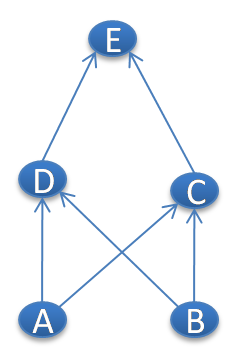
\includegraphics{exercises/figures/exercise1a-poset-D.png}
    \caption{Partially orderd set D}
    \label{img:ex1a:posetD}
  \end{center}
\end{figure} \\
Let there be two subsets S$_{1}$ = \{A, B, C\} and S$_{2}$ = \{A, B, D\} as displayed in Figures \subref{img:ex1a:subsetS1} and \subref{img:ex1a:subsetS2}.
\begin{figure}[htbp]
	\begin{center}
	 	\subfigure[Subset S$_{1}$]{
  	 	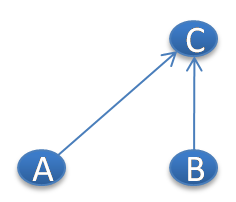
\includegraphics{exercises/figures/exercise1a-subset-S1.png}
   		\label{img:ex1a:subsetS1}
		}
		\subfigure[Subset S$_{2}$]{
   		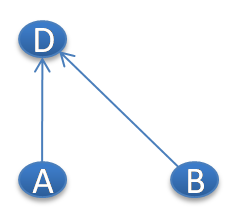
\includegraphics{exercises/figures/exercise1a-subset-S2.png}
	   	\label{img:ex1a:subsetS2}
		}
	\end{center}
\end{figure} \\
The union of S$_{1}$ and S$_{2}$ would not directed, be since (C, D) does not have an upper bound in $S_{1} \cup S_{2}$ as displayed in Figure \ref{img:ex1a:union}
\begin{figure}[htbp]
  \begin{center}
    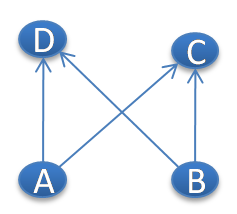
\includegraphics{exercises/figures/exercise1a-union-S1-S2.png}
    \caption{Union of S$_{1}$ and S$_{2}$}
    \label{img:ex1a:union}
  \end{center}
\end{figure}

\subsection{If $S_{1} \subseteq D$ and $S_{2} \subseteq D$ are directed, then so is $S_{1} \cap S_{2}$.}
\textbf{This statement is false}. Considering the two subsets S$_{1}$ and S$_{2}$ from 1a, the intersection would be \{A, B\} as displayed in Figure \ref{img:ex1b:intersection}. Obviously, these two elements do not have an upper bound in $S_{1} \cap S_{2}$.
\begin{figure}[htbp]
  \begin{center}
    
\includegraphics{exercises/figures/exercise1b-intersect-S1-S2.png}
    \caption{Intersection of S$_{1}$ and S$_{2}$}
    \label{img:ex1b:intersection}
  \end{center}
\end{figure}

\subsection{For every $d \in D$, the set $\{s \in D | s \leq d\}$ is directed.}
\textbf{This statement is true}:

Let $S$ be the set ${s \in D | s \leq d}$. \\
Since $\exists s \in S$ for each $s \in D$ where $s \leq d$ and because that $d \in D$ and $d \leq d$,

$\Rightarrow$ it must be that $d \in S$. \\
Also, for each $s \in S$

$\Rightarrow$ it must be that $s \leq d$.

$\Rightarrow$ Therefore, $d \geq \sqcup s$ for each $s \in S$.

$\Rightarrow$ Consequently $d \geq \sqcup (a, b)$ for each $(a, b) \in (S \times S)$, assuming that $x \geq \sqcup (y, z)$ if $x \geq \sqcup \{y, z\}$.


$\Rightarrow$ Hence, $d$ is upper bound to all two elements of $S$, thus making $S$ directed.

\subsection{For every $d \in D$, the set $\{s \in D | d \leq s\}$ is directed.}
\textbf{This statement if false}. Consider a poset D as displayed in Figure \ref{img:ex1d:posetD}
\begin{figure}[htbp]
  \begin{center}
    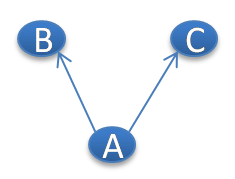
\includegraphics{exercises/figures/exercise1d-poset-D.png}
    \caption{Partially ordered set D}
    \label{img:ex1d:posetD}
  \end{center}
\end{figure}
The statement does allow choosing A for $d$ which would result in the entire poset. Consequently, the poset itself would need to be directed. Obviously, B and C have no upper bound, thus the poset is not directed.